\begin{figure}

\begin{subfigure}{\linewidth}

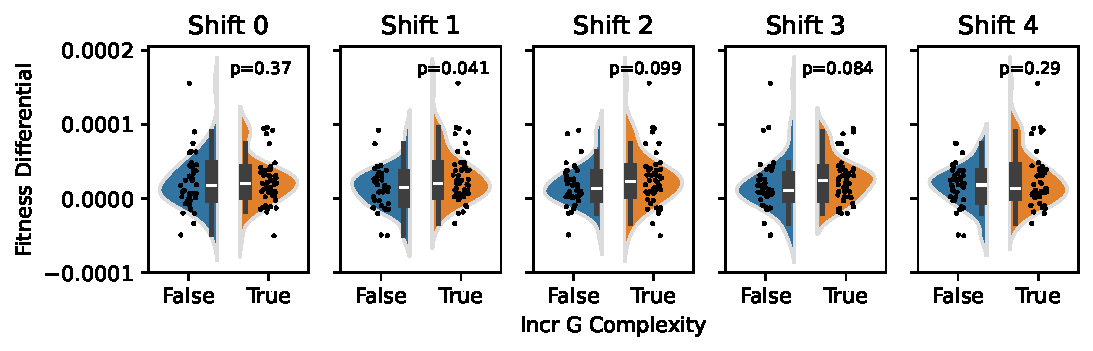
\includegraphics[width=\linewidth]{binder-2025-08-28-complexity-adaptation/binder/teeplots/2025-08-28-complexity-adaptation/how=shift+sign=-1+viz=subplots+ext=.pdf}
\caption{fitness differential value at forward-looking offset, "shift" corresponding to offset size}

\end{subfigure}

\vspace{2ex}

\begin{subfigure}{\linewidth}

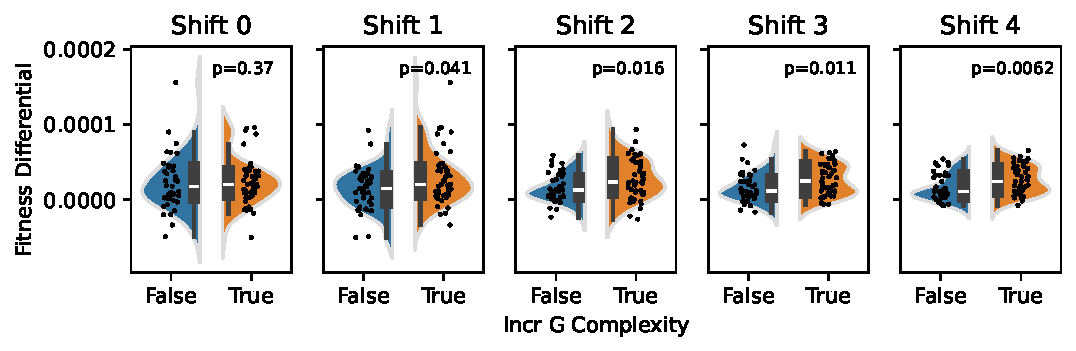
\includegraphics[width=\linewidth]{binder-2025-08-28-complexity-adaptation/binder/teeplots/2025-08-28-complexity-adaptation/how=rollingmean+sign=-1+viz=subplots+ext=.pdf}
\caption{fitness differential mean over forward-looking window, "shift" corresponding to window size}

\end{subfigure}

\vspace{1ex}

\caption{
\textbf{Backwards-looking control for Figure \ref{fig:potentiate}.}
Comparisons find no backwards-looking association between complexity and fitness gains (i.e., fitness gains driving subsequent complexity increase).
}
\label{fig:potentiate-control}

\end{figure}
